\documentclass{standalone}

\usepackage{tikz}
\usepackage{verbatim}

\usetikzlibrary{arrows}
\usetikzlibrary{calc}



\begin{document}

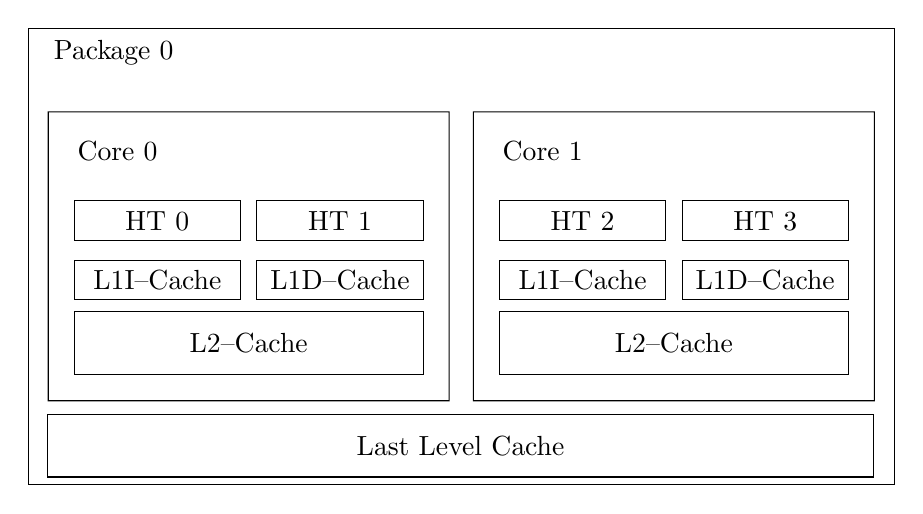
\begin{tikzpicture}[node distance=5mm, scale=2]

  % Colors
  % Styles
  \tikzstyle{package_style} =
    [font=\normalsize, text top left, text width=2cm, draw=black, shape=rectangle, inner sep = 1pt]
  \tikzstyle{thread_style} =
    [font=\normalsize, text centered, text width=1.9cm, draw=black,
    shape=rectangle, inner sep = 3pt, minimum width = 1cm, minimum height =.5cm]

  \tikzstyle{id_style} = [font=\normalsize, text centered, draw=none,
  color=black!60!white, rectangle]

  \tikzstyle{thread_shape} = \draw[thread_style];
  \tikzstyle{l1_cache_shape} = \draw[thread_style];
  \tikzstyle{l2_cache_shape} = [thread_style, minimum width = 4.43cm, minimum
    height =.8cm];

  % Drawing

  % First core
  \begin{scope}
    \node(l2)	[l2_cache_shape] {L2--Cache};
    \draw[transparent] (l2.west) -- +(0,4mm) coordinate(hi)[at end];
    \draw[transparent] (l2.east) -- +(0,4mm) coordinate(hd)[at end];

    \node(l1i)  [l1_cache_shape, right of=hi, anchor=west, node distance=0] {L1I--Cache};
    \node(l1d)  [l1_cache_shape, left of=hd, anchor=east, node distance=0] {L1D--Cache};

    \node(t0)	[thread_shape, above of=l1i, anchor=south] {HT 0};
    \node(t1)	[thread_shape, above of=l1d, anchor=south] {HT 1};

    \draw [transparent] (l2.south west) -- ++(-1mm,-1mm) node(swc) {};
    \draw [transparent] (l2.south east) -- ++(1mm,-1mm) node(sec) {};
    \draw [transparent] (t1.north east) -- ++(1mm,5mm) node(nec) {};
    \draw [transparent] (t0.north west) -- ++(-1mm,5mm) node(nwc) {};

    \draw[black] (swc.south west) -- (sec.south east) -- (nec.north east) --
    (nwc.north west) -- cycle;

    \node(core0) [anchor=north west] at (nwc.south east) {Core 0};
  \end{scope}

    \draw[transparent] (core0.north west) -- ++(0,5mm) coordinate(pid);
    \node(pack0) [rectangle, draw=none, anchor=west, xshift=-3mm] at (pid) {Package 0};

    % Package rectangle
%    \draw (-1.4cm,2.0cm) -- ++(0,-4.5cm) -- ++(5.5cm,0) -- ++(0,4.5cm) -- cycle;
    \draw (-1.4cm,2.0cm) -- ++(0,-2.9cm) -- ++(5.5cm,0) -- ++(0,2.9cm) -- cycle;

    % draw LLC
    \draw (-1.28cm,-.45) -- ++(5.25cm,0) -- ++(0,-.4cm) -- ++ (-5.25cm,0) -- cycle;
    \node(llc) at (1.345cm,-.65cm) {Last Level Cache};

%    \node(smt_id) [id_style, anchor=east, xshift=-11mm] at (t0.west) {SMT\_ID};
%    \draw[transparent] (smt_id.north) |- coordinate[midway](corner) (core0.west);
%    \node(core_id) [id_style] at (corner) {Core\_ID};

%    \draw[transparent] (core_id.north) |- coordinate[midway](pidc) (pid);
%    \node(package_id) [id_style] at (pidc) {Package\_ID};

%    \draw[transparent] (smt_id.south) |- coordinate[midway](cidc) (l1i.west);
%    \node(cid) [id_style] at (cidc) {L1--Cache\_ID};

%    \draw[transparent] (smt_id.south) |- coordinate[midway](cidc2) (l2.west);
%    \node(cid2) [id_style] at (cidc2) {L2--Cache\_ID};

  % Second core
  \begin{scope}[xshift=2.7cm]
    \node(1l2)	[l2_cache_shape] {L2--Cache};

    \draw[transparent] (1l2.west) -- +(0,4mm) coordinate(hi)[at end];
    \draw[transparent] (1l2.east) -- +(0,4mm) coordinate(hd)[at end];

    \node(1l1i)  [l1_cache_shape, right of=hi, anchor=west, node distance=0] {L1I--Cache};
    \node(1l1d)  [l1_cache_shape, left of=hd, anchor=east, node distance=0] {L1D--Cache};

    \node(1t0)	[thread_shape, above of=1l1i, anchor=south] {HT 2};
    \node(1t1)	[thread_shape, above of=1l1d, anchor=south] {HT 3};

    \draw [transparent] (1l2.south west) -- ++(-1mm,-1mm) node(1swc) {};
    \draw [transparent] (1l2.south east) -- ++(1mm,-1mm) node(1sec) {};
    \draw [transparent] (1t1.north east) -- ++(1mm,5mm) node(1nec) {};
    \draw [transparent] (1t0.north west) -- ++(-1mm,5mm) node(1nwc) {};

    \draw[black] (1swc.south west) -- (1sec.south east) -- (1nec.north east) --
    (1nwc.north west) -- cycle;

    \node(core1) [anchor=north west] at (1nwc.south east) {Core 1};
  \end{scope}

\begin{comment}
  % Third core
  \begin{scope}[yshift=-1.9cm]
    \node(2l2)	[l2_cache_shape] {L2--Cache};
    \node(2l1i)  [l1_cache_shape, above of=2l2, anchor=south east] {L1I--Cache};
    \node(2l1d)  [l1_cache_shape, above of=2l2, anchor=south west] {L1D--Cache};

    \node(2t0)	[thread_shape, above of=2l1i, anchor=south] {T 4};
    \node(2t1)	[thread_shape, above of=2l1d, anchor=south] {T 5};

    \draw [transparent] (2l2.south west) -- ++(-1mm,-1mm) node(2swc) {};
    \draw [transparent] (2l2.south east) -- ++(1mm,-1mm) node(2sec) {};
    \draw [transparent] (2t1.north east) -- ++(1mm,5mm) node(2nec) {};
    \draw [transparent] (2t0.north west) -- ++(-1mm,5mm) node(2nwc) {};

    \draw[black] (2swc.south west) -- (2sec.south east) -- (2nec.north east) --
    (2nwc.north west) -- cycle;

    \node(core2) [anchor=north west] at (2nwc.south east) {Core 2};
  \end{scope}

  % Fourth core
  \begin{scope}[xshift=2.7cm, yshift=-1.9cm]
    \node(3l2)	[l2_cache_shape] {L2--Cache};
    \node(3l1i)  [l1_cache_shape, above of=3l2, anchor=south east] {L1I--Cache};
    \node(3l1d)  [l1_cache_shape, above of=3l2, anchor=south west] {L1D--Cache};

    \node(3t0)	[thread_shape, above of=3l1i, anchor=south] {T 6};
    \node(3t1)	[thread_shape, above of=3l1d, anchor=south] {T 7};

    \draw [transparent] (3l2.south west) -- ++(-1mm,-1mm) node(3swc) {};
    \draw [transparent] (3l2.south east) -- ++(1mm,-1mm) node(3sec) {};
    \draw [transparent] (3t1.north east) -- ++(1mm,5mm) node(3nec) {};
    \draw [transparent] (3t0.north west) -- ++(-1mm,5mm) node(3nwc) {};

    \draw[black] (3swc.south west) -- (3sec.south east) -- (3nec.north east) --
    (3nwc.north west) -- cycle;

    \node(core3) [anchor=north west] at (3nwc.south east) {Core 3};
  \end{scope}
  \end{comment}
\end{tikzpicture}

\end{document}
